\documentclass[12pt,a4paper,oneside]{fithesis2}
\usepackage[slovak]{babel}       % Multilingual support
\usepackage[utf8]{inputenc}       % UTF-8 encoding
\usepackage[T1]{fontenc}          % T1 font encoding
\usepackage[                      % A sans serif font that blends well with Palatino
  scaled=0.86
]{berasans}
\usepackage[                      % A tt font if you do not like LM's tt
  scaled=1.03
]{inconsolata}
\usepackage[                      % Clickable links
  plainpages = false,               % We have multiple page numberings
  pdfpagelabels                     % Generate pdf page labels
]{hyperref}
\usepackage{blindtext}            % Lorem ipsum generator
\usepackage{amsmath}
\usepackage{dsfont}

\usepackage{listings}
\lstset{language=C++}
\usepackage{verbatimbox}
\usepackage{graphicx}
\parskip 1ex
\parindent 0in

\thesislang{sk}                   % The language of the thesis
\thesistitle{Vyhľadávanie najbližších vektorov s využitím knižnice FLANN}       % The title of the thesis
\thesissubtitle{Bakalárska práca}  % The type of the thesis
\thesisstudent{Tomáš Durčák}          % Your name
\thesiswoman{false}                % Your gender
\thesisfaculty{fi}                % Your faculty
\thesisyear{Jar \the\year}     % The academic term of your thesis defense
\thesisadvisor{RNDr. David Novák, Ph.D.}   % Your advisor

\begin{document}
  \FrontMatter                    % The front matter
    \ThesisTitlePage                % The title page
    \begin{ThesisDeclaration}       % The declaration
      \DeclarationText
      \AdvisorName
    \end{ThesisDeclaration}
    \begin{ThesisThanks}            % The acknowledgements (optional)
      I would like to thank my supervisor\,\dots
    \end{ThesisThanks}
    \begin{ThesisAbstract}          % The abstract
      The aim of the bachelor work is to provide\,\dots
    \end{ThesisAbstract}
    \begin{ThesisKeyWords}          % The keywords
      keyword1, keyword2\,\dots
    \end{ThesisKeyWords}
    \tableofcontents                % The table of contents
%   \listoftables                   % The list of tables (optional)
%   \listoffigures                  % The list of figures (optional)
  
  \MainMatter                     % The main matter
    \chapter{Úvod}          % Chapters
    V posledných dvoch desaťročiach sa do popredia stále viac a viac dostáva potreba vyhľadávania informácií v multimediálnych dátach, čo má za následok rapídny rozvoj technológií a metód v oblasti počítačového videnia (computer vision). Takýmito multimediálnymi dátami môže byť napríklad databáza obsahujúca množstvo obrázkov (rádovo v tisícoch, prípadne miliónoch). Bežnou požiadavkou užívateľa je vyhľadať 
v takejto databáze obrázky, ktoré sú podobné dotazu, teda obrázku, ktorý systému užívateľ ponúkne. Od tejto podobnosti sa očakáva, že výsledné obrázky vrátené ako výsledok budú obsahovať objekty podobné objektom na dotazovanom obrázku. Ďalej sa očakáva, že vyhľadávanie podobných obrázkov bude efektívne v rýchlosti výpočtu a podobnosti medzi obrázkami.

Problém nájdenia najbližšieho suseda (nearest neighbor search) má veľký význam pre rôzne aplikácie ako napríklad: rozpoznávanie obrazu, kompresiu dát, rozpoznávanie vzorov a ich klasifikáciu, strojové učenie, štatistiku a analýzu dát. Avšak, riešenie tohto problému vo vysoko dimenzionálnych priestoroch sa zdá byť zložitý problém. Toto viedlo k zvýšeniu záujmu o triedy vyhľadávacích algoritmov, ktoré dokážu riešiť tento problém rýchlejšie ako bežné algoritmy.

Pre túto úlohu existujú rôzne vyhľadávacie indexy a za jedno z najlepších riešení je považovaná knižnica FLANN\footnote{Fast Library for Approximate Nearest Neighbors}. Cieľom bakalárskej práce bolo túto knižnicu otestovať na rôznych dátach dodaných vedúcim a vyhodnotiť efektivitu vyhľadávania. Výsledky boli porovnané s výkonom indexovaných štruktúr vyvinutých v laboratóriu DISA\footnote{Laboratory of Data Intensive Systems and Applications, MU Fakulta informatiky, Brno}.

Plus tu dopíšem stručný popis jednotlivých kapitol..

    \chapter{Základné pojmy}
    
    	\section{Vektorový priestor}
    Vektorový priestor $ \Omega = D_1D_2. . .D_n $ má dimenziu $n$. Objekt (resp. vektor alebo bod)  $\mathcal{O} = [a_1, a_2, . . . , a_n] $ patriaci do vektorového priestoru je jednoznačne určený svojimi súradnicami $ a_i \in D_i, 1 \le i \le n, $ ktorých je práve $n$. $D_i$ je doménou dimenzie a určuje množinu hodnôt(resp. vlastností), ktoré môže príslušná vektorová súradnica nadobúdať \cite{stromy}.
    	
    Vektorový priestor $\Omega$, definujeme nad určitým poľom $\mathbf{P} $, s význačným prvkom $\mathbf{0}$ a dvomi binárnymi operáciami, sčítaním $+ : \Omega \times \Omega \rightarrow \Omega $  a násobením $\cdot : \mathbf{P}  \times \Omega \rightarrow \Omega$, takými že platí: 
     
\begin{equation*}
\forall u,v,w \in \Omega : (u + v)+w = u+(v+w) 
\end{equation*}
\begin{equation*}
\exists\mathbf{0} \in \Omega : u+\mathbf{0} = \mathbf{0}+u = u
\end{equation*}
\begin{equation*}
\forall u \in \Omega \; \exists \; u \in \Omega : u+(-u)  = \mathbf{0}
\end{equation*}
\begin{equation*}
\forall a,b \in \mathbf{P} \; \exists \; u \in \Omega : (a.b).u = a.(b.u) 
\end{equation*}
\begin{equation*}
\forall u \in \Omega : 1.u=u  \textrm{ kde } 1 \in \mathbf{P}  \textrm{ je jednotkový prvok z } \mathbf{P} 
\end{equation*}
\begin{equation*}
\forall a,b \in \mathbf{P} \; \exists \;u \in \Omega : (a+b).u = a.u + b.u 
\end{equation*}
\begin{equation*}
\forall a \in \mathbf{P} \; \exists \;u,v \in \Omega : a.(u+v) = a.u + a.v 
\end{equation*} \\
\textbf{Poznámka:} Vektorový podpriestor je tiež vektorový priestor.

\textbf{Príklad:}
Obrázok (resp. jeho histogram farieb) môže byť vektorom vo vektorovom priestore a mať súradnice podľa počtu pixelov z každého farebného odtieňu.
Potom vektor z histogramu farieb je:
\begin{equation*}
\{(\alpha_1,\beta_1),...(\alpha_M,\beta_M)\}
\end{equation*}
kde $M$ je počet farebných odtieňov. \\
Iným príkladom môže byť dokument reprezentovaný ako
vektor v $m$-rozmernom priestore príznakov, ktoré zodpovedajú jednotlivým slovám – tzv.termom. Množina $n$ dokumentov je reprezentovaná ako matica $n\times m$. Neplnovýznamové slová (pomocne slovesá, spojky...) sa zvyčajne odstránia \cite{vectorspace}. 

\begin{figure}[h']
  \centering
  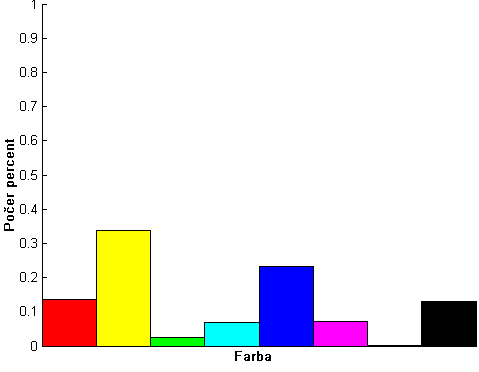
\includegraphics[width=5cm]{obr/histogram.png}
  \caption{Histogram farieb s ôsmimi farebnými odtieňmi. Zdroj:\cite{histogram}}
  \label{fig:triangle}
\end{figure}  

\textbf{Normovaný vektorový priestor}\\
Normovaný vektorový priestor je vektorový priestor nad $\mathbb{R}^n$, v ktorom je každému vektoru $x$ priradené reálne číslo - \textbf{norma}, vyjadrujúca dĺžku vektora $x$. \textbf{Normou} na reálnom vektorovom priestore $V$ rozumieme ľubovoľné zobrazenie $V \rightarrow \mathbb{R}$, ktoré vektoru $x \in V$ priradí reálne číslo $\| x \|$, také, že pre všetky $x,y \in V$ a ľubovoľné $c \in \mathbb{R}$ platí:
\begin{equation*}
\| x + y \| \leq \|x\| + \|y\|
\end{equation*}
\begin{equation*}
\| cx \| = |c| \| x \|
\end{equation*}
\begin{equation*}
\|x\| = 0  \Rightarrow x = 0
\end{equation*}
Reálny vektorový priestor s normou teda nazývame normovaný priestor. Intuitívne je to vektorový priestor, v ktorom možno merať dĺžky vektorov. \textit{Vzdialenosť bodov} $a, b$ vo vektorovom priestore $V$ s normou $\| \cdot \|$ nazývame dĺžku vektora $a - b$, teda číslo $\|a-b\|$.
    \section{Metrický priestor}
    
    Metrický priestor je množina, na ktorej je definovaná vzdialenosť pre všetky prvky z množiny. Táto vzdialenosť sa nazýva metrika. Metriku môžme definovať ako funkciu, ktorá určuje vzdialenosť medzi dvomi objektami. \\ \\
    \textbf{Definícia:} Nech $X\neq 0$ je množina. Definujme zobrazenie \\ $d: X \times X \rightarrow R $, ktoré spĺňa nasledujúce vlastnosti:
    \begin{align*}
    \textrm{ Pre všetky } x,y,z \in X \qquad d(x,x) &= 0 \\
    d(x,y) &\textgreater 0 \qquad x\neq y \\
    d(x,y) &= d(y,x) \\
    d(x,z) + d(z,y) &\geq d(x,y)
    \end{align*}
    
    Množinu \textbf{$X$} nazývame \textbf{základnou množinou}, zobrazenie $d$ \textbf{metrikou} a  dvojicu $(X,d)$ \textbf{metrickým priestorom}.
    V tej istej množine môžme definovať rôzne metriky. Metrika $d$ musí byť vždy nezáporná \cite{Yianilos:1993:DSA:313559.313789}. \\ \\
    \textbf{Príklad:} 
    Vzdialenosť dvoch bodov na priamke v $ \mathbf{R} \quad d=|x-y| $ alebo v rovine v
     $\mathbf{R^2} \quad d = \sqrt{(x_1-y_1)^2+(x_2-y_2)^2}$.
    
    \section{Metrické vs. vektorové priestory}
    
    Hoci pojmy \textit{vektorový} a \textit{metrický priestor} sú úplne odlišné, niektoré známe priestory ako napríklad $\mathbb{R}^3$, sú súčasne vektorové priestory aj metrické priestory. 
    
    Všeobecne platí, že v metrickom priestore niesu definované špeciálne operácie sčítania $+$ a skalárneho súčinu $\cdot$, ktoré sú vo vektorovom priestore. Na druhej strane, vo všeobecnosti vektorový priestor nemusí mať definovaný pojem "vzdialenosť".
    
    Normovaný vektorový priestor je automaticky metrický priestor, definovaním vzdialenosti medzi dvomi objektami. Každý metrický priestor však nemusí byť vektorovým priestorom.
    
	\section{Vzdialenostné funkcie}
	
	Vzdialenostné funkcie predstavujú hlavný spôsob určenia blízkosti alebo podobnosti dvoch objektov v určitej doméne. Táto vzdialenosť môže byť definovaná rôzne. Najčastejšie v závislosti od použitého dátového typu alebo účelu aplikácie.
	Vzdialenostné funkcie rozdeľujeme na dva základne typy podľa charakteru ich návratovej hodnoty:
	\begin{itemize}
	\item \textbf{diskrétne --} vracajú len vopred určenú množinu hodnôt malého rozsahu, napr. 	     len hodnotu $1$ alebo $-1$
	\item \textbf{spojité --} rozsah vrátenej množiny hodnôt je veľmi veľký alebo aj nekonečno, 		napr. hodnoty z intervalu $[0,1]$
	\end{itemize}
	Ďalej si popíšeme najčastejšie používané vzdialenostné funkcie. Jednu z nich budeme používať aj v testovaní a porovnávaní testovaných knižníc \cite{Zezula2, Chavez:2001}.
\subsection{Minkowského vzdialenosť}
Minkowského vzdialenosť je generalizovaná metrika, ktorá zahŕňa tzv. $L_p$ metriky v zovšeobecnenej forme. Minkowskí ju definoval takto: 
\begin{equation*}
L_p((x_1,...,x_n),(y_1,...,y_n))=\sqrt[p]{\left(\sum\limits_{i=1}^n \mid x_i-y_i \mid^p \right)}
\end{equation*}
Rovnica udáva vzdialenosť medzi dvomi objektami v $n$-dimenzionálnom priestore pre $p\geq 1$ (ak by bolo $p \textless 1$ nešlo by o metriku) \cite{Zezula2}.  \\
	\begin{figure}
  		\centering
  		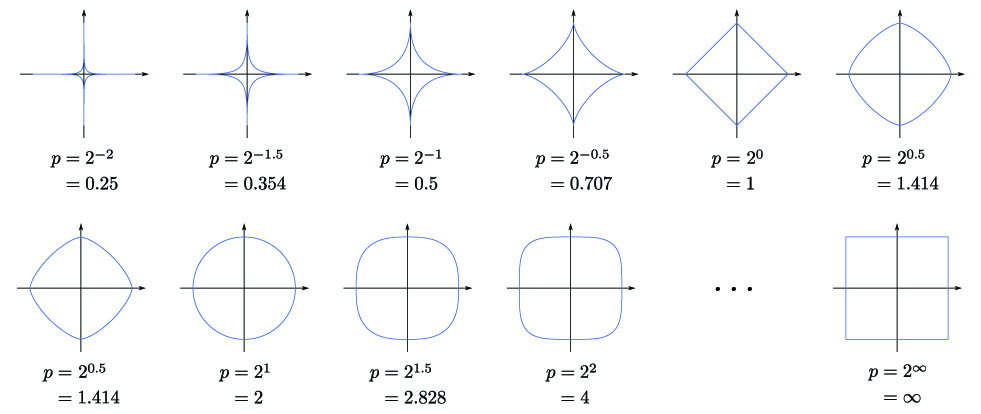
\includegraphics[width=\textwidth]{obr/lp.jpg}
  		\caption{Znázornenie $L_p$- metrík v $R^2$ podľa parametra p. Zdroj:\cite{lp}}
  		%\label{fig:triangle}
	\end{figure}  

Medzi najznámejšie a najpoužívanejšie metriky patria:
\begin{itemize}
\item $L_1$ -- Manhattanská metrika vyjadruje najkratšiu vzdialenosť, ktorú musíme prejsť aby sme sa v meste dostali z jedného bodu do druhého. Je pomenovaná podľa pravouhlého systému ulíc v meste New York.
\item $L_2$ -- Euklidovská metrika vyjadruje najkratšiu vzdušnú vzdialenosť medzi dvomi objektmi. $L_2$ je použitá aj pri testoch.
\item $L_\infty $ -- Čebyševova metrika, nazýva sa tiež maximálna alebo šachovnicová vzdialenosť, pretože na šachovnici, je to minimálny počet ťahov potrebných na prejdenie kráľom z jedného štvorca na iný.
\end{itemize}
   \section{Vyhľadávanie v metrických a vektorových priestoroch}
   Základnou charakteristikou vyhľadávania vo vektorových a metrických priestoroch je neurčitosť. Týka sa to hlavne problému \textbf{Nájdenia najbližšieho suseda} (ang. Nearest neighbor search) \cite{nns2009}. Tento problém obecne definujeme takto: \\
   Je daná množina bodov $P=\{p_1,...,p_n\}$ v priestore $X$ a dotazované body $q \in M$, nájdite najbližšie body z $P$ ku $q$.\\
   Pod pojmom \textbf{najbližší sused} rozumieme objekt alebo bod podobný dotazovanému bodu. Nepožadujeme aby boli výsledky vyhľadávania vždy na 100\% presné, ale aby výpočet skončil v čo najkratšom čase.
   Pred vyhľadávaním sa musíme rozhodnúť, ako chceme určovať blízkosť objektov, akú metriku použijeme. V našich testoch bola použitá $L_2$ metrika, čiže klasická Euklidovská metrika, ktorá je vhodná pre husto vzorkované dáta. Ďalej sa musíme rozhodnúť, koľko najbližších susedov budeme hľadať. Existujú 3 základné druhy dotazov:
   \begin{itemize}
   \item \textbf{Dotaz na najbližšieho suseda}- hľadáme najbližší najpodobnejší objekt k dotazu, výsledkom je 1 objekt ku každému dotazu.
   
   \textbf{Definícia:}
   \begin{equation*}
   NN(q)=\{x \in X, \forall y \in X| d(q,x)\leq d(q,y) \}
   \end{equation*}
Výsledkom je bod $x$, ktorého vzdialenosť od dotazu $q$ je najmenšia spomedzi všetkých bodov z množiny $X$.
   \item \textbf{Dotaz na k-najbližších susedov}- niekedy nám nemusí stačiť len 1 najbližší objekt, preto hľadáme $k$ susedov, ktorý sú mu podobný.
   
   \textbf{Definícia:}
   \begin{equation*}
   kNN(q)=\{A|A \subseteq X,|A|=k,\forall x \in A,\forall y \in X - A,d(q,x)\leq d(q,y)\}
   \end{equation*}    
   \item \textbf{Rozsahový dotaz}- použijeme, keď chceme nájsť všetkých najbližších susedov, ktorý su od dotazovaného bodu $q$ vzdialený maximálne zvolenú hodnotu $r$ (polomer vyhľadávania).
   
   \textbf{Definícia:} %R(q,r)=\{ x \in X|d(q,x)\leq r \}
   \begin{equation*} 
  rNN(q,X,r)=\{ x \in X|d(q,x)\leq r \}
   \end{equation*}  
   \end{itemize}
   
	\begin{figure}[h]
  		\centering
  		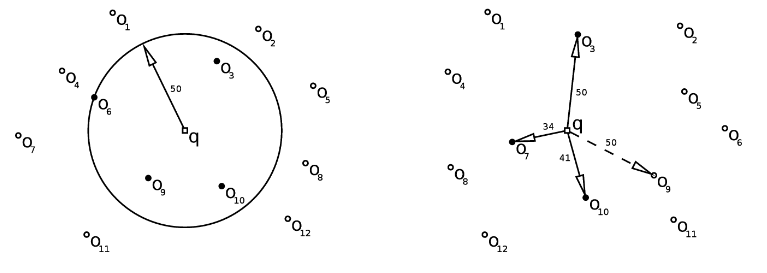
\includegraphics[width=10cm]{obr/knn.png}
  		\caption{Znázornenie $kNN$ a $rNN$ v $L_2$-metrike. Zdroj:\cite{knnPavelJurkas}}
  		\label{fig:rozdelenie priestoru}
	\end{figure}  

\section{Indexové štruktúry}

Pri vyhľadávaní v metrických alebo vektorových priestoroch je vhodné dáta rozdeliť do menších podmnožín a niektoré dáta pri prezeraní vynechať, čím sa môže odpoveď na dotaz značne urýchliť. Na roztriedenie dát používame špeciálne indexové štruktúry. Dve z nich si v podkapitolách popíšeme.
\subsection{KD-stromy}
KD = k-dimenzionálny strom \cite{Kibriya2007} je binárny strom slúžiaci na reprezentáciu priestorových dát vyšších dimenzií vo vektorovom priestore. Dáta sú v strome rozdeľované podľa viac-dimenzionálnych kľúčov, ktorými sú zvyčajne súradnice bodov alebo vektorov. \\ \\
\textbf{Vytvorenie KD-stromu}\\
\textbf{Vstup:} Množina objektov v k-dimenzionálnom priestore. \\
\textbf{Problém:} Vytvoriť strom, ktorý rozdeľuje priestor polrovinami, tzn. každý objekt je vo svojom vlastnom kvádri. Viď \ref{fig:polroviny}\\
\begin{figure}[h]
  		\centering
  		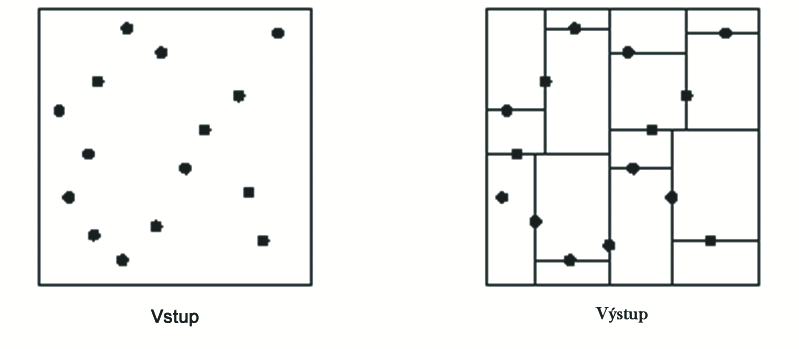
\includegraphics[width=9cm]{obr/lp2.png}
  		\caption{Rozdelenie priestoru na jednotlivé polroviny}
  		\label{fig:polroviny}
\end{figure}\\
\textbf{Samotná konštrukcia stromu:}
\begin{enumerate}
\item V každej úrovni stromu vyberáme postupne jeden z koordinátov $ \{ x_1,x_2,...,x_k \} $ ako základ rozdeľovania ostatných objektov. Napríklad v koreni stromu sa rozhodujeme podľa $x_1$ a ako v binárnom vyhľadávacom strome, všetky objekty s hodnotou koordinátu $x_1$ menšou ako hodnota koreňového uzlu budú v ľavom pod-strome a s väčšou alebo rovnou hodnotou budú v pravom pod-strom
\item V ďalšej pod-úrovniach stromu triedime objekty postupne podľa ďalších koordinátov, keď už bude mať strom hĺbku $k$, začíname porovnávať opäť od začiatku podľa $x_1,...$
\item Ak by sme vkladali objekty do stromu v náhodnom poradí, strom by bol nevyvážený, preto sa vkladané objekty vyberajú podľa priemernej hodnoty všetkých hodnôt na danom koordináte alebo podľa mediánu
\item Po log(n) krokoch sa rozklad zastaví, každý objekt má svoje miesto
\end{enumerate} 
\textbf{Vkladanie objektu do stromu:} \\
\textbf{Príklad:} Do stromu na Obr. \ref{fig:kdtree} vložíme objekt s kľúčom (11,8)
\begin{itemize}
\item V koreni sa podľa koordinátu $x$ porovná s uzlom (7,2), kedže 11>7 ide doprava
\item V ďalšej úrovní sa porovná podľa $y$ s uzlom (9,6), kedže 8>6 ide doprava, tento uzol je prázdny, preto sa na toto miesto uloží objekt (11,8)
\end{itemize}
\begin{figure}[h]
  		\centering
  		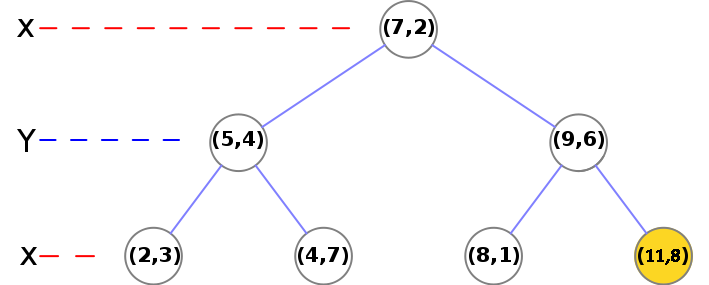
\includegraphics[width=7cm]{obr/kdtree01.png}
  		\caption{Vkladanie objektu do KD-stromu}
  		\label{fig:kdtree}
\end{figure}
\textbf{Vyhľadávanie v KD-strome} \\
KD-strom umožňuje vyhľadávať najbližšie body. Na Obr. \ref{fig:polroviny} je znázornené ako strom rozdelí vektorový priestor na menšie obdĺžniky (polroviny). Nájdenie najbližšieho objektu teda znamená nájdenie oblasti, v ktorej je dotaz $q$ a prehľadanie okolitých oblastí, kde by sa ešte mohol nachádzať ešte bližší bod.
\\
\textbf{Algoritmus:} 
\begin{itemize}
\item Nájde sa bunka $c$ obsahujúca objekt $q$
\item $q$ je ohraničená nejakým objektom $p$ (to ale nemusí byť najbližší objekt)
\item Nájdeme všetky najbližšie bunky $c'$ vo vzdialenosti $d(p,q)$
\item Otestujeme či $c'$ neobsahuje bližší objekt
\end{itemize}
\textbf{Použitie:}\\
KD-stromy sa používajú hlavne na indexovanie objektov s nižšou dimenziou. Pri vyšších dimenziách sa začne prejavovať tzv. \textit{prekliatie dimenzionality}, ktoré spôsobuje neefektívnosť pri vyhľadávaní.

  
\subsection{M-stromy}
   Pre indexovanie objektov v metrických priestoroch sa často využíva dátová štruktúra M-strom \cite{stromy}. Štruktúru stromu tvorí opäť n-arny strom ako u KD-stromu. Rozdiel spočíva v obsahu uzlov a listov stromu. Samotné objekty sú uložené len v listových uzloch stromu. Nelistové uzly obsahujú tzv. \textbf{smerovacie objekty}. \\\\
Každý smerovací objekt v uzle obsahuje:
\begin{itemize}
\item Samotný objekt $O_r$, ktorý môže byť \textit{virtuálny} -- vypočítaný pre účely M-stromu alebo \textit{skutočný} -- uložený v niektorom liste $T(O_r)$
\item Odkaz $ptr(T(O_r))$ n svoj pod-strom $T(O_r)$
\item Polomer $r(O_r)$
\item Vzdialenosť $d(O_r,P(O_r))$  od svojho rodičovského smerovacieho objektu $P(O_r)$
\end{itemize}
Listové uzly vypadajú podobne, ale miesto odkazu na svoj pod-strom a polomeru obsahujú $oid(O_j)$ -- identifikátor celého objektu.\\

Princíp hierarchie M-stromu spočíva rovnako ako u KD-stromu v rozdelení priestoru na menšie regióny, ktoré ale nemusia byť nutne disjunktné ako je to u KD-stromu. K rozdeleniu slúžia smerovacie objekty, pričom všetky objekty v listových uzloch, ktoré obsahuje pod-strom $T(O_r)$ smerovacieho objektu $O_r$, sú vo vzdialenosti maximálne $r(O_r)$ od $O_r$. Teda:
\begin{equation*}
\forall O_i \in T(O_r) \qquad   d(O_r,O_i) \leq r(O_r)
\end{equation*}
\begin{figure}
  		\centering
  		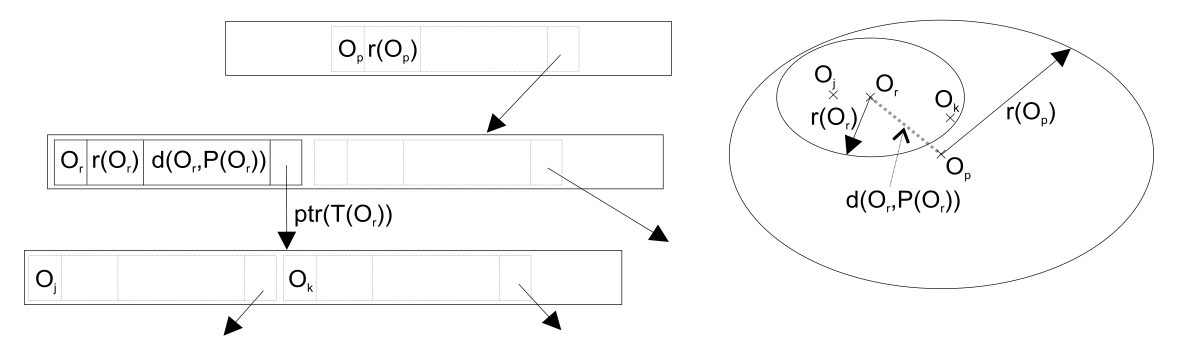
\includegraphics[width=13cm]{obr/m-tree.png}
  		\caption{Uzly M-stromu obsahujúce objekty (vľavo) a regióny smerovacích objektov znázornené v metrickom priestore (vpravo)} Zdroj: \cite{stromy} 
  		%\label{fig:triangle}
  		\label{m-strom}
\end{figure}
Na obrázku \ref{m-strom} je znázornená štruktúra stromu a vzťahy medzi smerovacími objektami.\\
\\
\textbf{Vytvorenie M-stromu:}\\
Rovnaká množina objektov môže byť v M-strome indexovaná mnohými rôznymi spôsobmi, pričom neporušíme ani jeden z axiomov metriky alebo vlastnosti M-stromov. Avšak každý z týchto spôsobov nemusí byť práve ideálny z hľadiska efektivity operácií vykonávaných nad M-stromom. Obecne hľadáme také spôsoby konštrukcie stromov, aby zložitosť dotazovanie bola minimálna. Efektívnosť vyhľadávania v značnej miere ovplyvňuje výber smerovacích objektov tzv. \textit{pivotov}, ktoré potrebujeme na rozdelenie metrického priestoru pri vytváraní stromu. Dôležitý je vyber pivotov, ktorí sú vo vhodnej vzdialenosti od ostatných objektov. Dobrí pivoti by mali byť navzájom ďaleko od seba a taktiež by sa mali nachádzať ďaleko od ostatných objektov v metrickom priestore. \\
\\
\textbf{Vyhľadávanie v M-strome:}\\
V M-stromoch môžme vyhľadávať \textit{k-najbližších susedov} ako aj pomocou \textit{rozsahového dotazu}. 

Pri vyhľadávaní k-najbližších susedov je dôležitá prioritná rada, z ktorej postupne vyberáme objekty na vyhľadávanie v strome $T(O_r)$. Každý objekt v rade má tvar:\\ $(prt(T(O_r)), d_{min}(T(O_r)))$. Prvý člen je už známy ukazateľ na pod-strom, druhý člen je spodná hranica medzi dotazovaným objektom $Q$ a každým objektom $O_j$ z $T(O_r)$.
\\ \\
\textbf{Použitie:} \\
M-stromy požívame, keď dáta nie je možné indexovať vo vektorovom priestore, alebo keď sú vektory dát príliš dlhé (dimenzia \textgreater \,20). Metrický priestor umožňuje definovať špeciálne metriky a tým rôzne interpretovať vzdialenosť (resp. podobnosť) objektov na základe ich vlastností.

	\chapter{Knižnica FLANN}
	FLANN\footnote{Z anglického: Fast Library for Approximate Nearest Neighbors} je knižnica poskytujúca rýchly programátorsky nástroj, ktorý slúži na \textit{vyhľadávanie najbližších susedov}. Pre tento účel obsahuje kolekciu nástrojov (algoritmov) a tiež systém automatického výberu najlepšieho algoritmu a optimálnych parametrov použitých pri vyhľadávaní najbližších susedov. Aby bolo vyhľadávanie čo najrýchlejšie, je knižnica FLANN napísaná v programovacom jazyku C++ a je možné ju použiť aj pri programovaní v jazykoch C, Matlab, Python a Ruby. Knižnica je voľne šíriteľná pod licenciou BSD\footnote{BSD licencia sa používa pre voľne šíriteľný softvér, je pomenovaná podľa Berkeley Software Distribution, Unixový operačný systém} \cite{flann_pami_2014}.
	
V ďalších podkapitolách si popíšeme algoritmy 
\textit{The Multiple Randomized kd-trees}\footnote{Algoritmus náhodných KD-stromov},
\textit{The Priority Search K-Means Tree}\footnote{Algoritmus pre prioritné K-means stromy} a 
\textit{The Hierarchical Clustering Tree\protect\footnote{Algoritmus pre Hierarchické zhlukovacie stromy}}, ktoré sú obsiahnuté v knižnici FLANN a javia sa najrýchlejšie z pomedzi existujúcich algoritmov na vyhľadávanie najbližších susedov.
	\section{Algoritmus Náhodných KD-stromov}
Klasické algoritmy využívajúce KD-stromy sú vhodné na vyhľadávanie najbližších susedov v nízko-dimenzionálnych dátach, avšak pre vyššie dimenzie vykazujú značný pokles výkonu. Tento problém viedol k vývoju nového a vylepšeného algoritmu využívajúceho KD-stromy. \cite{flann_pami_2014}	
	
	Algoritmus je založený na stavaní mnohopočetných náhodných KD-stromov, ktoré sú prehľadávané paralelne. Originálne KD-stromy pri vytváraní delia dáta na polovicu v každej úrovni stromu vždy postupne podľa dimenzií zaradom. Na porovnanie náhodne KD-stromy vyberajú deliacu dimenziu náhodne z prvých $D$ dimenzií, kde majú dáta najväčší rozptyl. Knižnica FLANN používa v implementácií algoritmu hodnotu $D$ = 5, ktorá sa pri testoch ukázala ako optimálna. Pri vyhľadávaní sa používa prioritná rada skrz všetky randomizované KD-stromy. Objekty v tejto rade sú zoradené podľa zvyšujúcej sa vzdialenosti od deliacej hranice v každej úrovni, čo zvyšuje rýchlosť vyhľadávania. Každý objekt, ktorý už bol porovnaný s dotazom v niektorom strome, je označený a v ďalších  stromoch sa už neporovnáva. Presnosť aproximácie vyhľadávania sa reguluje nastavením maximálneho počtu listových uzlov (skrz všetky stromy), ktoré sa pri vyhľadávaní skontrolujú \cite{flann_pami_2014}.	
	
	\section{Algoritmus pre Prioritné K-means stromy}
	Pri niektorých typoch dát, môže byť efektívnejší algoritmus K-means stromov, zvlášť ak je prioritou vysoká presnosť výsledkov. Algoritmus prioritných K-means stromov sa snaží lepšie využívať prirodzenú štruktúru vstupných dát. Na rozdiel od randomizovaných KD-stromov, delí a zoskupuje dáta do skupín za základe vzdialeností skrz všetky dimenzie, pričom KD-stromy využívajú na delenie v každej úrovni len jeden rozmer \cite{flann_pami_2014}.
	
	\textbf{Opis algoritmu:}\\
	Pri tvorení K-means stromu sa dáta delia v každej úrovni do $K$ rôznych regiónov pomocou \textit{K-means zhlukovacieho algoritmu}. Rovnaká metóda sa rekurzívne aplikuje na každú novú skupinu dát. Delenie končí, keď počet objektov v každom regióne je menší ako hodnota $K$ \cite{flann_pami_2014}. %Presnejší popis a štruktúra algoritmu v \cite{flann_pami_2014}.
	
	\textbf{Výhľadávanie v strome:}\\
	K-means strom sa prehľadáva postupne od koreňa k najbližšiemu listu. Vetvy, ktoré boli pri prechádzaní stromu preskočené sa ukladajú do prioritnej rady, zoradené podľa vzdialenosti k dotazovanému objektu. Algoritmus potom ešte skontroluje pod-stromy uložené v tejto rade \cite{flann_pami_2014}. %Presnejší náhľad algoritmu je opäť v \cite{flann_pami_2014}.
	
	Počet regiónov $K$, na ktoré sa vstupné dáta delia pri vytváraní stromu určuje parameter algoritmu nazvaný \textit{počet vetiev stromu}. Výber optimálneho $K$ ovplyvňuje rýchlosť a správnosť vyhľadávania. Ďalším parametrom je $I_{max}$ a určuje maximálny počet iterácií, ktoré sa vykonajú pri delení stromu na regióny. Menší počet iterácií urýchli stavbu stromu, ale zníži presnosť vyhľadávania. Posledným parametrom je výber algoritmu, ktorý určí ako sa bude počítať rozhodovacia hranica pri delení objektov do regiónov. K dispozícií mame: \textit{náhodný výber}, \textit{Gonzalesov algoritmus} (výber objektov, ktoré su ďaleko od seba)\cite{flann_pami_2014} alebo \textit{KMeans++ algoritmus} \cite{K-means++}.
	\section{Algoritmus pre Hierarchické zhlukovacie stromy}
	Prechádzajúce dva algoritmy sú určené predovšetkým na vyhľadávanie najbližších susedov vo vektorových dátach. Niesu však vhodné na vyhľadávanie v binárnych dátach. Pre tento účel bol vyvinutý nový algoritmus, ktorý využíva novú dátovú štruktúru: \textit{hierarchické zhukovacie stromy} \cite{Attach:binary_matching_crv2012}.
	
	Vytváranie hierarchického zhlukovacieho stromu je podobné K-means stromu.   Zo vstupných dát sa náhodne vyberie $K$ \textit{zhlukovacích centier} a objekty sa rozdelia do $K$ zhlukov podľa toho, ku ktorému zhlukovaciemu centru sú najbližšie. Hodnota $K$ je vstupný parameter algoritmu. Delenie potom prebieha rekurzívne na všetkých nových zhlukoch, až kým nie je počet objektov v zhluku menši ako $K$. Vtedy sa vytvoria listové uzly stromu \cite{Attach:binary_matching_crv2012}.
	
	Na rozdiel od algoritmu pre prioritné K-means stromy, nevytvárame zo vstupných dát len jeden strom, ale celý les stromov, v ktorom sa vyhľadáva paralelne. Aby bolo vytváranie stromov rýchlejšie, je výhodné vyberať zhukovacie centrá náhodne, pričom nedochádza k výraznému poklesu presnosti. Vyhľadávanie je podobné algoritmu pre K-means stromy \cite{Attach:binary_matching_crv2012}.
	
	Pred vytváraním stromu môžme nastaviť \textit{rozvetvenie stromu ($K$)}, \textit{počet stromov}, \textit{maximálny počet objektov v listových uzloch} a \textit{algoritmus pre výber prvých $K$ zhukovacích centier} \cite{Attach:binary_matching_crv2012}.
	
	\section{Automatický výber vyhľadávacích parametrov}\label{sec:autotuning}
	Výber správneho algoritmu a optimálnych parametrov pri vyhľadávanie najbližších susedov nie je triviálny problém. Správny voľba závisí od niekoľkých faktorov ako napríklad: štruktúra vstupných dát a zvolená presnosť vyhľadávania. Každý z možných algoritmov má množinu nastaviteľných parametrov, ktoré v značnej miere ovplyvňujú výsledky vyhľadávania. Je to napríklad počet náhodných stromov pri použití KD-stromu alebo počet vetiev každého uzla pri hierarchickom K-means strome \cite{muja_flann_2009}.
	
	Výber algoritmu je optimalizačný problém, ktorým sa snažíme nájsť najlepšie riešenie. Cenu výpočtu počítame ako kombináciu času potrebného na vyhľadávanie dotazov, času za ktorý sa vytvorí vyhľadávací index (strom) a pamäťovej záťaže. Každý z týchto faktorov má inú váhu v závislosti na aplikácií a použití. Ak vytvárame vyhľadávací index len raz, ale vyhľadávanie prebieha mnohokrát, je dôležitejší čas vyhľadávania ako čas potrebný na vytvorenie indexu. Niekedy vyhľadávame v indexe len raz, napríklad pri on-line aplikáciach, vtedy potrebujeme aby sa index vytvoril čo najrýchlejšie. Môžu nastať aj situácie, kedy potrebuje čo najmenšie pamäťová zaťaženie.Váha pamäťového zaťaženie je $w_m$ a váha času vytvorenie indexu je $w_b$. Celkovú cenu počítame pomocou:
	\begin{equation}
	\mathrm{cost} = \dfrac{s + w_bb}{(s + w_bb)}_{opt} + w_mm
	\label{cena}
	\end{equation}
kde $s$ je čas vyhľadávania a $b$ je čas potrebný na vytvorenie vyhľadávacieho indexu. Parameter $m = m_t/m_d$ reprezentuje pomer pamäte použitej na uloženie indexu ($m_t$) a uloženia dát ($m_d$). Parameter $w_b$ reguluje čas potrebný na vytvorenie indexu vzhľadom ku času vyhľadávania. Ak nastavíme $w_b = 0$, znamená to, že chceme čo najrýchlejšie vyhľadávať a nezaujíma nás rýchlosť vytvorenia indexu. Nastavením $w_b = 1$, priradíme času vyhľadávania a vytvorenia indexu rovnakú dôležitosť. Podobne $w_m$ nastavuje prioritu medzi časom (čas vyhľadávania vytvorenia indexu) a pamäťou, ktorú využíva vyhľadávací index. Hodnota $w_m \textless 1$ kladie väčšiu váhu na čas nehľadiac na pamäť a hodnota $w_m \textgreater 1$  kladie prioritu na množstvo využitej pamäte. Nastavením $w_m = 1$ priradíme rovnakú prioritu času aj využitiu pamäte \cite{muja_flann_2009}. 

Výber najlepšieho algoritmu a optimálnych parametrov sa vykonáva v dvoch krokoch: V prvom kroku vyberáme algoritmus s najlepšími výsledkami podľa rovnice \ref{cena}. Pri testovaní sa využívajú hodnoty z množiny \{1,4,8,16,32\} ako počet náhodných KD-stromov, \{1,5,10,15\} ako počet iterácií a \{16,32,64,128,256\} ako počet vetiev v K-means strome. V druhom kroku sa využíva Nelder-Mead downhill simplex metóda \cite{NelderMead65}, pomocou ktorej sa určia optimálne parametre pre algoritmus vybraný v prvom kroku. Optimalizácia môže byť počítaná na celých vstupných dátach, alebo len na časti. Typicky stačí $5-10\,\%$ a výsledky sa stále veľmi blížia optimálnym hodnotám (ak sú dáta podobnej štruktúry) \cite{muja_flann_2009}.

	\section{Použitie knižnice FLANN v C++}
	Jadro knižnice FLANN je naprogramované v programovacom jazyku C++, preto je na jej samotnú kompiláciu potrebný C++ prekladač. Knižnicu je možne použiť s Linuxovými distribúciami, ale aj Windowsom a OS X. Pre viac-jadrovú podporu je nutné mať nainštalovanú knižnicu OpenMP. Predkompilovanú knižnicu FLANN je  možné použiť aj pomocou knižnice PCL (Point Cloud Library)\footnote{http://www.pointclouds.org}, do ktorej je implementovaná jedna zo starších verzií. V ďalších častiach si popíšeme niektoré základné triedy a funkcie knižnice \cite{manual}.
	
	Na ukladanie dát slúži trieda \texttt{Matrix<ElementType>}. Ukladáme do nej vstupné objekty, dotazy a výsledky vyhľadávania(vzdialenosti a ID objektov). FLANN potrebuje mať všetky dáta v operačnej pamäti. Na načítanie dát, môže byť použitá knižnica HDF5\footnote{https://hdfgroup.org/HDF5/}, ktorá musí byť nainštalovaná pred kompiláciou knižnice FLANN. 
	
	Po načítaní dát, je potrebné vytvoriť vyhľadávací index a nastaviť parametre. Na tento účel slúži trieda \texttt{flann::Index<T>}. V konštruktore triedy sa nastavuje typ vzdialenostnej funkcie a typ vyhľadávacieho algoritmu. Medzi zakladné typy patrí:
	\begin{itemize}
	\item \textbf{LinearIndexParams} Určený pre lineárne vyhľadávanie.
	
	\item \textbf{KDTreeIndexParams} Index s týmto typom vytvorí randomizované KD-stromy, ktoré sa prehľadávajú paralelne. V štruktúre je možné nastaviť počet stromov (\texttt{trees}), ktoré sa majú vytvoriť. 

	\item \textbf{KMeansIndexParams} Index s týmto typom vytvorí hierarchický k-means strom.

	\item \textbf{CompositeIndexParams} Index s týmto typom je kombináciou randomizovaných KD-stromov a hierarchického K-means stromu. 

	\item \textbf{KDTreeSingleIndexParams} Index s týmto typom vytvorí jeden KD-strom, ktorý je optimalizovaný na vyhľadávanie v nízkodimenzionálnych dátach (napríklad 2D a 3D priestor).

	\item \textbf{KDTreeCuda3dIndexParams} Index s týmto typom vytvorí jeden KD-strom. Vytvorenie a vyhľadávanie v strome prebieha na CUDA kompatibilných grafických kartách. Tento typ indexu sa hodí na vyľadávanie veľkého počtu dotazov.
	
	\item \textbf{HierarchicalClusteringIndexParams} Index s týmto typom použíje na vyhľadávanie hierarchické zhlukovacie stromy.

	\item \textbf{AutotunedIndexParams} Tento typ indexu je určený pre automatický výber najlepšej vyhľadávacej štruktúry a jej optimálnych parametrov.
	
	\end{itemize}

Po výbere parametrov sa index vytvorí volaním metódy \texttt{buildIndex}. Vytvorenie indexu zvyčajne trvá dlhšiu dobu, preto je možné pre opätovné použitie vytvorený index uložiť do súboru.
Objekty sa dajú do indexu pridávať a odoberať aj po jeho vytvorení pomocou metód: \texttt{addPoints} a \texttt{removePoint}. 

Na samotné vyhľadávanie najbližších objektov k dotazom slúžia dve základné metódy:

\begin{itemize}
	\item \textbf{flann::Index::knnSearch} Slúži na vyhľadávanie K-najbližších susedov pre množinu dotazovaných objektov. Metóda má parameter \texttt{checks}, ktorý určuje počet listových uzlov, ktoré sa majú skontrolovať a môže byť nastavená na špeciálne hodnoty:\\ \texttt{FLANN\_CHECKS\_UNLIMITED} (skontroluje všetky listové uzly),\\ \texttt{FLANN\_CHECKS\_AUTOTUNED} (použije vypočítanú hodnotu, ak bol index vytvorený automaticky).

	\item \textbf{flann::Index::radiusSearch} Metóda na rozsahové vyhľadávanie najbližších objektov do vzdialenosti polomeru \texttt{radius} \cite{manual}. 

\end{itemize}

		

    \chapter{Porovnanie knižnice FLANN a M-indexu}
    Našim cieľom je porovnanie výkonu dvoch programovacích knižníc určených na vyhľadávanie najbližších susedov. Meranie výkonu programu zvyčajne zahŕňa niekoľko aspektov. Pre programy na vyhľadávanie najbližších susedov je to:
    \begin{itemize}
    \item celkový čas potrebný na vytvorenie indexu
    \item čas samotného vyhľadávania
    \item presnosť vyhľadávania
\end{itemize}   
Pre správnosť a férovosť porovnania je taktiež dôležite dodržať niekoľko zásad:
\begin{itemize}
\item Porovnávať výkon indexov podobnej veľkosti, napr. 4GB a 5GB. Zvyčajne nieje možne vytvoriť indexy úplne rovnakej veľkosti. Nie je však vhodné porovnávať 4GB index s 50GB indexom.

\item Ak počítame zrýchlenie oproti lineárnemu vyhľadávaniu, ktorá ma presnosť 100\% a čas vyhľadávania 100s, nemôžeme povedať, že vyhľadávanie s iným indexom, ktoré má presnosť 50\% a trvá 10s má zrýchlenie 10x, pretože presnosť nieje rovnaká ani podobná. Reálne môžme predpokladať, že vyhľadávanie hrubou silou bude trvať 50s, ak ma byť presnosť 50\%. Takže index je asi len 5x rýchlejší.

\item Pri porovnávaní sa často zabúda na zohľadnenie času, za ktorý sa vytvorí index, aj keď to môže byť jeden z najdôležitejších porovnávacích faktorov.
\end{itemize}
  
\section{Nastavenie parametrov}
\begin{description}

\item \textbf{Testovacie dáta:} súbory 100K, 300K, 500K a 1M 4096-dimenzionálnych vektorov, textový formát v zip archíve, každý objekt je uložený na dvoch riadkoch, prvý riadok obsahuje ID objektu(10 miestne číslo) samotný vektor je na ďalšom riadku atď.

\item \textbf{Dotazované objekty:} 1000 náhodne vybraných objektov z testovaných dát. 

\item \textbf{Groundtruth(správne výsledky):} 1000 najbližších susedov spočítaných pre každý dotaz, osobitne pre všetky testovacie dáta. Formát: 2 riadky pre každý dotaz, prvý riadok ID dotazu, druhý riadok 1000 párov(L2 vzdialenosť od dotazu, ID objektu), výsledky pre každý dotaz sú usporiadané podľa vzdialenosti.

\item \textbf{Parametre vyhľadávania:} \\
k=1, 10, 100 ,1000 \\
rôzne nastavenia presnosti vyhľadávania \\

\item \textbf{Merania:}
Presnosť vyhľadávania určuje: 
\begin{equation*}
\textrm{recall} =  \frac{ \textrm{odpoveď} \cap \textrm{groundtruth}}{k}
\end{equation*}
Meriame čas pre jeden dotaz, ako priemer z 1000 dotazov v [ms].

\item 
\end{description}


\section{Výsledky}
    \chapter{Záver}
    
\bibliographystyle{unsrt}
\bibliography{citacie}{}

    % Bibliography goes here
    % Index goes here (optional)
\end{document}
